\chapter{Summer School on Effective HPC for Climate and Weather -- 2020}
\label{ch:ss2020}

\section{Introduction}

The Summer School on Effective HPC for Climate and Weather has brought together young researchers and software engineers interested in the current technological developments in the field of climate modelling. Together, they explored hot topics in high-performance computing and climate and weather applications.

Making effective use of HPC environments becomes increasingly challenging for PhD students and young researchers. As their primary intent is to generate insight, they often struggle with the technical nature of the tools and environments that enable their computer-aided research: computation, integration, and analysis of relevant data. The scope of this event was the training of young researchers and software engineers in methods, tools, and theoretical knowledge to make effective use of HPC environments and generate insights for the field and their research.

While the school aimed to prepare the attendees for large scale simulation runs and data processing, it also covered a representative selection of modern concepts such as machine learning, domain-specific languages, containerisation, and analysis of climate/weather data using Python. The event also provided an outlook of challenges and strategies for HPC for climate and weather. Additionally, it was an opportunity to foster networking among scientists bringing together users of specific models and tools and enabling them to exchange their knowledge.

Due to COVID-19 restrictions, the Summer School 2020 was held as an online-only event from 24 to 28 of August, 2020. For more accessible communication, all participants were registered to our \href{https://hps.vi4io.org/mailman/listinfo/hps-summer-school}{mailing list}. For further information about the event, check the \href{https://hps.vi4io.org/events/2020/esiwace-school}{official webpage}.

We provided a \href{https://docs.google.com/document/d/1f9dDjTSnaCtGoJNQYa8eb3U6jCjQ_rjmVsDSo16cRzk/edit?usp=sharing}{Tutorial} to set up a Virtual Machine (VM) with Ubuntu and all the software for the training and lab sessions pre-installed. Participants were asked to set up the VM on their PC before the summer school to fully participate in the tutorial sessions and perform most of the training.

A certificate of attendance was provided to all participants that attend the event regularly. The Blackboard Collaborate stored the log details of every person connected to the event, and this information was used to select the participants that were worthy of a certificate.

The summer school supports the mission of the European Network for Earth System modelling (ENES). ENES is developing a common climate and Earth system modelling distributed research infrastructure in Europe integrating the European community on Earth's climate System Models (ESMs) and their hardware, software, and data environments.

The overarching goals of ENES are to:

\begin{itemize}

\item Further integrate the European climate modelling community;

\item Ease the development of full ESMs;

\item Foster the execution and exploitation of high‐end simulations;

\item Support the dissemination of model results and the interaction with the climate change impact community.

\end{itemize}

\section{Structure}

The ESiWACE Summer School was structured along with topical sessions in the morning/afternoon, from Monday to Thursday, a Q\&A session on Friday morning and a Keynote Talk on Friday afternoon.

A topical session typically consists of an academic lecture, and it may contain hands-on/lab practicals. Experts in the respective field organised each of these sessions.

The hands-on tutorials/lab practicals worked as follows:

\begin{itemize}

\item A video tutorial was pre-recorded and provided an introduction/walk-through to the topic.

\item The tutorials were scheduled for each session, but the usage was up to the participant's discretion.

\item We provide a tutorial to set up a Virtual Machine (VM). The VM comes with Ubuntu and all the software for the training pre-installed. Attendees may install the VM on their PC to perform most of the training. Some training may be on a dedicated cluster. You should set up the VM before the summer school if you like to participate in the tutorial sessions.

\item A lab practical may list additional exercises and suggestions for further learning.

\item At the end of the day, a time slot for a Virtual Lab Session is given to allow independent and self-paced learning, and participants can decide what and when they want to engage.

\end{itemize}

On Friday, the dedicated Q\&A slot per lab practical was scheduled. The session offered the participants the opportunity to contact the organiser of each hands-on session and ask questions regarding the topic and particularly regarding the tutorial and exercises.

Throughout the event, additional support was provided by the mailing list, in which participants may have posted questions and cooperated with other students and the organisers.

All sessions were recorded and the recordings, together with the presentations and material for each session, were made available in the main summer school webpage.

\section{Topics and Sessions}

The topics covered in the summer school were:

\begin{itemize}

\item Extreme-Scale Computation -- Section \ref{sec:esc}

\item Parallel Programming in Practice -- Section \ref{sec:ppp}

\item Modern Storage -- Section \ref{sec:me}

\item Input/Output and Middleware -- Section \ref{sec:ioam}

\item Machine Learning -- Section \ref{sec:ml}

\item ECMWF -- Virtual Visit -- Section \ref{sec:ECMWF}

\item High-Performance Data Analytics and Visualisation -- Section \ref{sec:hpdaav}

\item Performance Analysis -- Section \ref{sec:pa}

\item Containers -- Section \ref{sec:c}

\end{itemize}

On Friday, we organised a Q\&A session a Keynote Talk:

\begin{itemize}

\item Q/A Session -- Section \ref{sec:qas}

\item Keynote Talk -- Section \ref{sec:kt}

\end{itemize}

\subsection{Extreme-Scale Computation}
\label{sec:esc}

\subsubsection{Abstract}

This session will introduce the concept of extreme-scale computing with an explanation of the trends in the computer architectures that provide the underlying computing power. In particular, the increasing use of parallelism and heterogeneity in these architectures will be discussed.

A high-level overview will then be given of the performance, portability and productivity (3P's) requirements that Weather and Climate models have to run successfully on these computer architectures. It will be shown how current approaches can struggle to meet all three of these requirements.

Lastly, a relatively new, Domain-Specific Language (DSL), approach to programming Weather and Climate models will be introduced with examples from two existing DSLs - DAWN and PSyclone. It will be shown that the DSL approach offers the possibility of supporting all three of the above requirements, by separating the implementation of the science code from its parallelisation and optimisation on the underlying computer architecture.

\subsubsection{Learning Objectives}

\begin{itemize}

\item Illustrate the complexity and diversity of extreme-scale computing on examples in climate and weather
\item State the Performance, Portability and Productivity requirements of Weather and Climate models (3P's)
\item Describe how Domain-Specific Languages (DSLs) can provide a solution to the problem of providing the 3P's
\item Use PSyclone and Gridtools DSLs for small applications

\end{itemize}

\subsubsection{Sessions}

\begin{table}[H]
\begin{center}
\begin{tabular}{|l|l|l|}
\hline
\multicolumn{3}{|c|}{\textbf{Extreme-Scale Computation}} \\ \hline
\multicolumn{3}{|l|}{Chair: Rupert Ford (STFC, UK)} \\
\multicolumn{3}{|l|}{Chair: Carlos Osuna (MeteoSwiss, Switzerland)} \\ \hline \hline
Time & \multicolumn{1}{c|}{Title} & \multicolumn{1}{c|}{Speakers} \\ \hline \hline
09:00 & Extreme Computing Session - Overview & Rupert Ford \\ \hline
09:05 & Supercomputer Trends & Simon McIntosh-Smith \\ \hline
09:30 & Performance, Portability and Productivity & Rupert Ford \\ \hline
10:00 & Introduction to DSLs & Ben Weber and Rupert Ford \\ \hline
10:45 & An Introduction to PSyclone & Andrew Porter \\ \hline
11:15 & Dusk \& Dawn - Introduction and Overview & Giacomo Serafini \\ \hline
11:45 & Tutorial Introduction & Carlos Osuna \\ \hline
12:15 & Lab Tutorial: Extreme-Scale Computation & \\ \hline
      & PSyclone Tutorial & \\ \hline
      & Dusk \& Dawn Tutorial & \\ \hline
\end{tabular}
\end{center}
% \caption{Schedule of the session Extreme-Scale Computation. Note that the titles are links to the presented material.}
\end{table}

\slidetable
{summer-school-ec0_overview}
{https://hps.vi4io.org/_media/events/2020/summer-school-ec0_overview.pdf}
{https://www.youtube.com/watch?v=aZ8J7fqWd7M&list=PL_PBXYC_ExoP_hNaiBvvbt8y1sbbShroH&index=3&t=0s}
{Extreme Computing Session - Overview}
{0.35}

\slidetable
{summer-school-esiwace2_mcintosh-smith_aug_2020}
{https://hps.vi4io.org/_media/events/2020/summer-school-esiwace2_mcintosh-smith_aug_2020.pdf}
{https://www.youtube.com/watch?v=VVw8U_nTQ1g&list=PL_PBXYC_ExoP_hNaiBvvbt8y1sbbShroH&index=4&t=0s}
{Supercomputer Trends}
{0.26}

\slidetable
{summer-school-ec2_ppp}
{https://hps.vi4io.org/_media/events/2020/summer-school-ec2_ppp.pdf}
{https://www.youtube.com/watch?v=pXz3io7rHw4&list=PL_PBXYC_ExoP_hNaiBvvbt8y1sbbShroH&index=5&t=0s}
{Performance, Portability and Productivity}
{0.35}

\slidetable
{summer-school-ec3_dslintro}
{https://hps.vi4io.org/_media/events/2020/summer-school-ec3_dslintro.pdf}
{https://www.youtube.com/watch?v=qhLsGvMVccU&list=PL_PBXYC_ExoP_hNaiBvvbt8y1sbbShroH&index=6&t=0s}
{Introduction to DSLs}
{0.35}

\slidetable
{summer-school-ec4_psycloneintro}
{https://hps.vi4io.org/_media/events/2020/summer-school-ec4_psycloneintro.pdf}
{https://www.youtube.com/watch?v=t6mK2zRWkJI&list=PL_PBXYC_ExoP_hNaiBvvbt8y1sbbShroH&index=7&t=0s}
{An Introduction to PSyclone}
{0.35}

\slidetable
{summer-school-dawn_intro}
{https://hps.vi4io.org/_media/events/2020/summer-school-dawn_intro.pdf}
{https://www.youtube.com/watch?v=zcgFJhhWHlQ&list=PL_PBXYC_ExoP_hNaiBvvbt8y1sbbShroH&index=8&t=0s}
{Dusk \& Dawn - Introduction and Overview}
{0.35}

\slidetable
{summer-school-psyclonetutorialintro}
{https://hps.vi4io.org/_media/events/2020/summer-school-psyclonetutorialintro.pdf}
{}
{PSyclone Tutorial}
{0.35}

\slidetable
{summer-school-dawntutorialintro}
{https://hps.vi4io.org/_media/events/2020/summer-school-dawntutorialintro.pdf}
{}
{Dusk \& Dawn Tutorial}
{0.35}

\subsubsection{Comments from the Survey}

``I found it quite hard to follow, but I like the idea of different half an hour topics."

``The use of Anaconda for the PSyclone tutorial was a really helpful and interactive tool!"

\subsection{Parallel Programming in Practice}
\label{sec:ppp}

\subsubsection{Abstract}

In this session, we will provide a global overview of how the main concepts of parallel programming are implemented in weather and climate codes. We will detail the different parallel programming models for distributed and shared memory systems and describe the resulting scalability of commonly-used algorithms implementing those models.

Particular attention will be devoted to specific features that may inhibit scaling and performance of weather and climate codes. This analysis will be done at the level of the code routine itself but also in the more general context of code coupling, the latter being a specific implementation of coarse grain parallelism.

\subsubsection{Learning Objectives}

\begin{itemize}

\item Describe the scaling characteristics of commonly used algorithms in weather and climate models
\item Discuss issues which may inhibit scaling and performance
\item Classify programming models for distributed and shared memory systems
\item Identify performance features and potential issues for computer processor architectures
\item Describe the concepts of coupling software
\item Classify coupling software implementations given their main characteristics
\item Evaluate qualitatively the impact of different coupling configurations (sequential vs concurrent, multi vs mono-executable, etc.) on coupled model performance
\item Describe the most used coupling software in climate and weather applications

\end{itemize}

\subsubsection{Sessions}

\begin{table}[H]
\begin{center}
\begin{tabular}{|l|l|l|}
\hline
\multicolumn{3}{|c|}{\textbf{Parallel Programming in Practice}} \\ \hline
\multicolumn{3}{|l|}{Chair: Sophie Valcke (Cerfacs, France)} \\
\multicolumn{3}{|l|}{Chair: Christopher Maynard (University of Reading, UK)} \\ \hline \hline
Time & \multicolumn{1}{c|}{Title} & \multicolumn{1}{c|}{Speakers} \\ \hline \hline
13:30 & Scaling Algorithms & Christopher Maynard \\ \hline
15:15 & Code Coupling & Sophie Valcke \\ \hline
\end{tabular}
\end{center}
\end{table}

\slidetable
{summer-school-cmm_scale_compressed}
{https://hps.vi4io.org/_media/events/2020/summer-school-cmm_scale_compressed.pdf}
{https://www.youtube.com/watch?v=lWI3LDfYGTE&list=PL_PBXYC_ExoP_hNaiBvvbt8y1sbbShroH&index=8&t=0s}
{Scaling Algorithms}
{0.35}

\slidetable
{summer-school-svalcke_esiwace2}
{https://hps.vi4io.org/_media/events/2020/summer-school-svalcke_esiwace2.pdf}
{https://www.youtube.com/watch?v=AnMmr1HvP1I&list=PL_PBXYC_ExoP_hNaiBvvbt8y1sbbShroH&index=9&t=0s}
{Code Coupling}
{0.35}

\subsection{Modern Storage}
\label{sec:me}

\subsubsection{Abstract}

\subsubsection{Learning Objectives}

\begin{itemize}

\item Describe the architecture and architectural implications of modern storage architectures and object stores suitable for extreme-scale computing
\item Discuss the storage stack with its semantics and potential performance implications on different levels: in particular POSIX vs MPI-IO vs NetCDF and high-level I/O middleware
\item Execute the Darshan tool to identify I/O patterns and assess the performance
\item Apply benchmarking tools to assess the performance

\end{itemize}

\subsubsection{Sessions}

\begin{table}[H]
\begin{center}
\begin{tabular}{|l|l|l|}
\hline
\multicolumn{3}{|c|}{\textbf{Modern Storage}} \\ \hline
\multicolumn{3}{|l|}{Chair: Sai Narasimhamurthy (Seagate, UK)} \\
\multicolumn{3}{|l|}{Chair: Jean-Thomas Acquaviva (DDN, France)} \\ \hline \hline
Time & \multicolumn{1}{c|}{Title} & \multicolumn{1}{c|}{Speakers} \\ \hline \hline
09:00 & Modern Storage & Sai Narasimhamurthy, \\
      &                & Konstantinos Chasapis \\ \hline
10:45 & Lab Tutorial: Modern Storage & \\ \hline
      & Darshan Demonstration - Hands-on Session & Konstantinos Chasapis \\ \hline
      & Installing Darshan for I/O Performance Analysis & Konstantinos Chasapis \\ \hline
      & Introduction to Using Darshan for I/O & Konstantinos Chasapis \\
      & Performance Analysis                  &  \\ \hline
\end{tabular}
\end{center}
\end{table}

\slidetable
{summer-school-modern-storage-esiwace}
{https://hps.vi4io.org/_media/events/2020/summer-school-modern-storage-esiwace.pdf}
{https://www.youtube.com/watch?v=Ph4EKiJ4LVk&list=PL_PBXYC_ExoP_hNaiBvvbt8y1sbbShroH&index=11&t=4s}
{Modern Storage}
{0.35}

\slidetable
{summer-school-darshan}
{https://hps.vi4io.org/_media/events/2020/summer-school-darshan.pdf}
{https://www.youtube.com/watch?v=c5inY63Ars0&list=PL_PBXYC_ExoP_hNaiBvvbt8y1sbbShroH&index=12&t=0s}
{Darshan Demonstration - Hands-on Session}
{0.35}

\slidetable
{modern-storage}
{}
{https://www.youtube.com/watch?v=sw1zi4biOVQ&list=PL_PBXYC_ExoOoNzLAVGTd0tg_KfwtV-Sf&index=3&t=41s}
{Installing Darshan for I/O Performance Analysis}
{0.35}

\slidetable
{modern-storage}
{}
{https://www.youtube.com/watch?v=8NWW5SJLjL0&list=PL_PBXYC_ExoOoNzLAVGTd0tg_KfwtV-Sf&index=4&t=51s}
{Introduction to Using Darshan for I/O Performance Analysis}
{0.35}

\subsubsection{Comments from the Survey}

``All the session was overall interesting. Konstantinos' presentation was great; the constant interruptions by his colleague, however, was a little disturbing."

\subsection{Input/Output and Middleware}
\label{sec:ioam}

\subsubsection{Abstract}

Climate and weather research is typically data-intensive, and applications must utilise input/output efficiently. Often, a user struggles to assess observed performance leading to superflux attempts to tune the application and optimise performance in a wrong layer of the stack.

The content of this session is twofold. Firstly, we discuss storage layers focusing on the NetCDF middleware and provide a performance model that aids users to identify inefficient I/O. Secondly, we introduce the NetCDF Climate and Forecast (CF) conventions that are often used as a standard to exchange data.

\subsubsection{Learning Objectives}

\begin{itemize}

\item Discuss challenges for data-driven research
\item Describe the role of middleware and file formats
\item Identify typical I/O performance issues and their causes
\item Apply performance models to assess and optimise I/O performance
\item Design a data model for NetCDF/CF
\item Analyse, manipulate and visualise NetCDF data
\item Execute programs in C and Python that read and write NetCDF files in a metadata-aware manner
\item Implement an application that utilises parallel I/O to store and analyse data
\item Describe ongoing research activities in high-performance storage

\end{itemize}

\subsubsection{Sessions}

\begin{table}[H]
\begin{center}
\begin{tabular}{|l|l|l|}
\hline
\multicolumn{3}{|c|}{\textbf{Input/Output and Middleware}} \\ \hline
\multicolumn{3}{|l|}{Chair: Julian Kunkel (University of Reading, UK)} \\
\multicolumn{3}{|l|}{Chair: Luciana Pedro (University of Reading, UK)} \\ \hline \hline
\multicolumn{3}{|l|}{Chair: Sadie Bartholomew (University of Reading, UK)} \\ \hline \hline
Time & \multicolumn{1}{c|}{Title} & \multicolumn{1}{c|}{Speakers} \\ \hline \hline
13:30 & Input/Output and Middleware & Luciana Pedro \\ \hline
15:15 & Python Data Tools for CF-netCDF & Sadie Bartholomew \\ \hline
16:45 & Lab Tutorial: Input/Output and Middleware & \\ \hline
      & An Introduction to NetCDF Using C Language & Luciana Pedro \\ \hline
      & CF-NetCDF with cfdm, cf-python and cf-plot & Sadie Bartholomew \\ \hline
\end{tabular}
\end{center}
\end{table}

\slidetable
{summer-school-talk-io}
{https://hps.vi4io.org/_media/events/2020/summer-school-talk-io.pdf}
{https://www.youtube.com/watch?v=0SdhJ7tiHEM&list=PL_PBXYC_ExoP_hNaiBvvbt8y1sbbShroH&index=12&t=0s}
{Input/Output and Middleware}
{0.6}

\slidetable
{summer-school-cfnetcdf}
{https://hps.vi4io.org/_media/events/2020/summer-school-cfnetcdf.pdf}
{https://www.youtube.com/watch?v=sCiX1djITYA&list=PL_PBXYC_ExoP_hNaiBvvbt8y1sbbShroH&index=13&t=0s}
{Python Data Tools for CF-netCDF}
{0.5}

\slidetable
{summer-school-lab-io-c}
{https://hps.vi4io.org/_media/events/2020/summer-school-lab-io-c.pdf}
{https://www.youtube.com/watch?v=L-BOT--meTw&list=PL_PBXYC_ExoOoNzLAVGTd0tg_KfwtV-Sf&index=4&t=7s}
{An Introduction to NetCDF Using C Language}
{0.6}

\slidetable
{cf-training}
{}
{https://www.youtube.com/watch?v=cqZnJm6_2sA&list=PL_PBXYC_ExoOoNzLAVGTd0tg_KfwtV-Sf&index=6&t=0s}
{CF-NetCDF with cfdm, cf-python and cf-plot}
{0.4}

\subsubsection{Comments from the Survey}

``I really liked both presentations."

``I enjoyed a lot this session, was really descriptive! I would have liked to have this session before the Modern Storage session to be able to have a better understanding."

``The lab session was awesome. I learned so much."

``Sadie gave an exceptional lab session of the Python data tools for CF-netCDF. A lot of great tools and libraries to use."

\subsection{Machine Learning}
\label{sec:ml}

\subsubsection{Abstract}

(1) Predicting weather and climate require modelling the Earth System -- a huge system that consists of many individual components that show chaotic behaviour and for which conventional tools often struggle to provide satisfying results.

(2) A huge amount of data of the Earth System is available from both observations and modelling.

(3) Machine learning methods allow learning complex non-linear behaviour from data if enough data is available and to apply the learned tools efficiently on modern supercomputers.

If you combine (1), (2) and (3), it is easy to see that there are a large number of potential application areas for machine learning in weather and climate science that are currently explored. However, whether these approaches will succeed is still unclear as there are also a number of challenges for the application of machine learning tools in weather predictions.

This talk will provide an introduction to machine learning, outline how to apply machine learning in Earth System modelling, show examples for the application of machine learning throughout the weather and climate modelling workflow, and discuss the challenges that will need to be tackled.

\subsubsection{Learning Objectives}

\begin{itemize}

\item Describe the relevance of Machine Learning and its application to judge why there is such a hype around the topic at the moment
\item Explore how machine learning can be used in weather and climate modelling
\item List several specific examples for the use of machine learning at ECMWF
\item Discuss challenges for machine learning in weather and climate science

\end{itemize}

\subsubsection{Sessions}

\begin{table}[H]
\begin{center}
\begin{tabular}{|l|l|l|}
\hline
\multicolumn{3}{|c|}{\textbf{Machine Learning}} \\ \hline
\multicolumn{3}{|l|}{Chair: Peter Dueben (ECMWF, UK)} \\ \hline \hline
Time & \multicolumn{1}{c|}{Title} & \multicolumn{1}{c|}{Speakers} \\ \hline \hline
09:30 & Machine Learning for Weather and Climate Predictions & Peter Dueben \\ \hline
\hline
\end{tabular}
\end{center}
\end{table}

\slidetable
{summer-school-machine-learning}
{https://hps.vi4io.org/_media/events/2020/summer-school-machine-learning.pdf}
{https://www.youtube.com/watch?v=NgL-MDZbgIk&list=PL_PBXYC_ExoP_hNaiBvvbt8y1sbbShroH&index=14&t=0s}
{Machine Learning for Weather and Climate Predictions}
{0.3}

\subsection{ECMWF -- Virtual Visit}
\label{sec:ECMWF}

\subsubsection{Computer Hall Tour}

Learn about the performance and specifications of the ECMWF High-Performance Computing Facilities, and the way this supercomputer is used for operations, storage and research by ECMWF and its 34 Member \& Co-operating States.

The presentation will include a video tour of the computing facilities currently located in our HQ in Reading and a preview of what the new data centre will look like when it opens in Bologna (Italy) next year.

\subsubsection{Weather Room Tour}

Learn about ECMWF Forecasting products and activities. A member of the ECMWF Forecasting team will introduce you to the maps, charts and plots that are produced daily in the ``Weather Room" for weather prediction and analysis.

\subsubsection{Sessions}

\begin{table}[H]
\begin{center}
\begin{tabular}{|l|l|l|}
\hline
\multicolumn{3}{|c|}{\textbf{ECMWF -- Virtual Visit}} \\ \hline
\multicolumn{3}{|l|}{Chair: Peter Dueben (ECMWF, UK)} \\ \hline \hline
Time & \multicolumn{1}{c|}{Title} & \multicolumn{1}{c|}{Speakers} \\ \hline \hline
11:00 & Introduction to ECMWF & Peter Dueben \\ \hline
11:30 & Computer Hall Tour & Umberto Modigliani \\ \hline
12:00 & Weather Room Tour & David Lavers \\ \hline
\hline
\end{tabular}
\end{center}
\end{table}

\slidetable
{summer-school-ecmwf-general-overview}
{https://hps.vi4io.org/_media/events/2020/summer-school-ecmwf-general-overview.pdf}
{https://www.youtube.com/watch?v=HVKpKZtxd6I&list=PL_PBXYC_ExoP_hNaiBvvbt8y1sbbShroH&index=15&t=0s}
{Introduction to ECMWF}
{0.3}

\slidetable
{summer-school-ecmwf-computer-hall-tour}
{https://hps.vi4io.org/_media/events/2020/summer-school-ecmwf-computer-hall-tour.pdf}
{https://www.youtube.com/watch?v=X6D4uDWYzgo&list=PL_PBXYC_ExoP_hNaiBvvbt8y1sbbShroH&index=16&t=0s}
{Computer Hall Tour}
{0.3}

\slidetable
{summer-school-ecmwf-weather-room-tour}
{https://hps.vi4io.org/_media/events/2020/summer-school-ecmwf-weather-room-tour.pdf}
{https://www.youtube.com/watch?v=nV5MrZXMXsM&list=PL_PBXYC_ExoP_hNaiBvvbt8y1sbbShroH&index=17&t=0s}
{Weather Room Tour}
{0.3}

\subsubsection{Comments from the Survey}

``That was very interesting."

\subsection{High-Performance Data Analytics and Visualisation}
\label{sec:hpdaav}

\subsubsection{Abstract}

Analysis and visualisation of scientific data, such as those in the field of climate and weather, requires solution capable of effectively and efficiently handling massive data.

In this session, we will discuss some of the main challenges concerning scientific data management and in particular, those related to data analytics and visualisation. Software solutions for high-performance data analytics and visualisation, as well as examples of applications of these systems for real use cases in the climate and weather domain, will be presented.

The lab tutorial will provide a more practical introduction about some tools and modules for data analysis and how to apply these on climate data, as well as a walk-through of the VMI for the virtual lab.

\subsubsection{Learning Objectives}

\begin{itemize}

\item Discuss the main challenges of joining big data and HPC for scientific data management, in particular for data analytics and visualisation
\item Put into action practical hints about some HPDA tools and their application to scientific data at scale
\item Apply techniques and knowledge acquired during the course to real case studies in the weather and climate domain

\end{itemize}

\subsubsection{Sessions}

\begin{table}[H]
\begin{center}
\begin{tabular}{|l|l|l|}
\hline
\multicolumn{3}{|c|}{\textbf{High-Performance Data Analytics and Visualisation}} \\ \hline
\multicolumn{3}{|l|}{Chair: Donatello Elia (CMCC, Italy)} \\
\multicolumn{3}{|l|}{Chair: Niklas Röber (DKRZ, Germany)} \\ \hline \hline
Time & \multicolumn{1}{c|}{Title} & \multicolumn{1}{c|}{Speakers} \\ \hline \hline
13:30 & Data Visualization Using ParaView & Niklas Röber \\ \hline
14:00 & Hands-on: Data Visualization Using ParaView & \\ \hline
15:15 & High-Performance Data Analytics and Visualisation & Donatello Elia, \\
      &                                                   & Sandro Fiore \\
      &                                                   & (CMCC, Italy) \\ \hline
16:45 & Lab Tutorial: High-Performance Data Analytics & \\
      & and Visualisation                             & \\ \hline
      & High-Performance Data Analytics and Visualisation & Donatello Elia \\ \hline
\hline
\end{tabular}
\end{center}
\end{table}

\slidetable
{summer-school-visualizationdkrz}
{https://hps.vi4io.org/_media/events/2020/summer-school-visualizationdkrz.pdf}
{https://www.youtube.com/watch?v=XOoLgJp5RDs&list=PL_PBXYC_ExoP_hNaiBvvbt8y1sbbShroH&index=18&t=0s}
{Data Visualization Using ParaView}
{0.35}

\slidetable
{paraview-hands-on}
{}
{https://www.youtube.com/watch?v=jzOEVWWgb9c&list=PL_PBXYC_ExoOoNzLAVGTd0tg_KfwtV-Sf&index=7&t=0s}
{Hands-on: Data Visualization Using ParaView}
{0.35}

\slidetable
{summer-school-hpda_esiwace2_2020}
{https://hps.vi4io.org/_media/events/2020/summer-school-hpda_esiwace2_2020.pdf}
{https://www.youtube.com/watch?v=UF23BXfBQQs&list=PL_PBXYC_ExoP_hNaiBvvbt8y1sbbShroH&index=20&t=0s}
{High-Performance Data Analytics and Visualisation}
{0.35}

\slidetable
{summer-school-tutorial-high-performance_data_analytics_and_visualisation}
{https://hps.vi4io.org/_media/events/2020/summer-school-tutorial-high-performance_data_analytics_and_visualisation.pdf}
{https://www.youtube.com/watch?v=INoSZYXsX3Q}
{High-Performance Data Analytics and Visualisation}
{0.35}

\subsubsection{Comments from the Survey}

``This session was very good explained and very easy to follow."

\subsection{Performance Analysis}
\label{sec:pa}

\subsubsection{Abstract}

\subsubsection{Learning Objectives}

\begin{itemize}

\item Define performance analysis fundamentals (objectives, methods, metrics, hardware counters, etc.)
\item Describe the BSC performance analysis tools suite (Extrae, Paraver, Dimemas)
\item Interpret uses cases from Earth System Models (IFS, NEMO, etc.) that illustrate how to identify and solve performance issues
\item Apply profiling techniques to identify performance bottlenecks in your code
\item Summarise typical performance problems
\item Discuss specific knowledge about performance analysis applied to earth system modelling

\end{itemize}

\subsubsection{Sessions}

\begin{table}[H]
\begin{center}
\begin{tabular}{|l|l|l|}
\hline
\multicolumn{3}{|c|}{\textbf{Performance Analysis}} \\ \hline
\multicolumn{3}{|l|}{Chair: Mario C. Acosta (BSC, Spain)} \\
\multicolumn{3}{|l|}{Chair: Xavier Yepes (BSC, Spain)} \\ \hline \hline
Time & \multicolumn{1}{c|}{Title} & \multicolumn{1}{c|}{Speakers} \\ \hline \hline
09:00 & Computational Profiling Analysis for Climate and Weather & Xavier Yepes, \\
      &                                                          & Mario C. Acosta \\ \hline
10:45 & Lab Tutorial: Performance Analysis & \\ \hline
      & Paraver Hands-on Using the HARMONIE Model & Mario C. Acosta, \\
      &                                           & Xavier Yepes \\ \hline
\hline
\end{tabular}
\end{center}
\end{table}

\slidetable
{summer-school-2020_profilinganalysis}
{https://hps.vi4io.org/_media/events/2020/summer-school-2020_profilinganalysis.pdf}
{https://www.youtube.com/watch?v=fQ4w53T0qow&list=PL_PBXYC_ExoP_hNaiBvvbt8y1sbbShroH&index=21&t=0s}
{Computational Profiling Analysis for Climate and Weather}
{0.35}

\slidetable
{summer-school-2020_performance_analysis_hands-on}
{https://hps.vi4io.org/_media/events/2020/summer-school-2020_performance_analysis_hands-on.pdf}
{https://www.youtube.com/watch?v=HBvEG6RgHeE&list=PL_PBXYC_ExoOoNzLAVGTd0tg_KfwtV-Sf&index=10&t=0s}
{Performance Analysis: Paraver Hands-on Using the HARMONIE Model}
{0.35}

\subsection{Containers}
\label{sec:c}

\subsubsection{Abstract}

This session will present an introduction to an end-to-end scientific computing workflow utilising Docker containers. Attendees will learn about the fundamentals of containerisation and the advantages it brings to scientific software. Participants will then familiarise with Docker technologies and tools, discovering how to manage and run containers on personal computers, and how to build applications of increasing complexity into portable container images. Particular emphasis will be given to software resources which enable highly-efficient scientific applications, like MPI libraries and the CUDA Toolkit.

The second part of the lecture will focus on deploying Docker images on high-end computing systems, using a container engine capable of leveraging the performance and scalability of such machines, while maintaining a consistent user experience with Docker.

\subsubsection{Learning Objectives}

\begin{itemize}

\item Describe the difference between a container and a virtual machine
\item Explain the relationship between a container and a container image
\item Outline the basic workflow for the distribution of an image
\item List advantages of using containers for scientific applications
\item Write a Dockerfile
\item Build a container image using Docker
\item Run containers on personal computers using Docker
\item Perform basic management of Docker containers and images
\item Explain the motivations which drove the creation of HPC-focused container solutions
\item Highlight differences and similarities between Docker and Sarus

\end{itemize}

\subsubsection{Sessions}

\begin{table}[H]
\begin{center}
\begin{tabular}{|l|l|l|}
\hline
\multicolumn{3}{|c|}{\textbf{Containers}} \\ \hline
\multicolumn{3}{|l|}{Chair: Alberto Madonna (ETH Zürich, Switzerland)} \\
\multicolumn{3}{|l|}{Chair: Simon Wilson (NCAS, UK)} \\ \hline \hline
Time & \multicolumn{1}{c|}{Title} & \multicolumn{1}{c|}{Speakers} \\ \hline \hline
13:30 & Introduction to Containers and Docker & Alberto Madonna \\ \hline
15:15 & Introduction to Containers on HPC & \\
      & with the Sarus Container Engine & Alberto Madonna \\ \hline
16:45 & Lab Tutorial: Containers & \\ \hline
      & Containers Hands-on & \\ \hline
\hline
\end{tabular}
\end{center}
\end{table}

\slidetable
{summer-school-docker_introduction}
{https://hps.vi4io.org/_media/events/2020/summer-school-docker_introduction.pdf}
{https://www.youtube.com/watch?v=_04WSw9J6bI&list=PL_PBXYC_ExoP_hNaiBvvbt8y1sbbShroH&index=22&t=0s}
{Introduction to Containers and Docker}
{0.25}

\slidetable
{summer-school-sarus_introduction}
{https://hps.vi4io.org/_media/events/2020/summer-school-sarus_introduction.pdf}
{https://www.youtube.com/watch?v=1stRdcdVOEw&list=PL_PBXYC_ExoP_hNaiBvvbt8y1sbbShroH&index=23&t=0s}
{Introduction to Containers on HPC with the Sarus Container Engine}
{0.25}

\slidetable
{summer-school-docker-step-by-step}
{https://hps.vi4io.org/_media/events/2020/summer-school-docker-step-by-step.pdf}
{https://www.youtube.com/watch?v=dv74sFb3cVc&list=PL_PBXYC_ExoOoNzLAVGTd0tg_KfwtV-Sf&index=9&t=627s}
{Containers Hands-on}
{0.35}

\subsubsection{Comments from the Survey}

``Unfortunately, I was lost with the topic."

\subsection{Q/A Session}
\label{sec:qas}

\subsubsection{Abstract}

On Friday, a dedicated Q\&A slot per lab practical was scheduled. The session offered the participants the opportunity to contact the organiser of each hands-on session and ask questions regarding the topic and particularly regarding the tutorial and exercises.

\subsubsection{Sessions}

\begin{table}[H]
\begin{center}
\begin{tabular}{|l|l|l|}
\hline
\multicolumn{3}{|c|}{\textbf{Q/A Session (CHAIRS TO BE DOUBLE-CHECKED.)}} \\ \hline
\multicolumn{3}{|l|}{Chair: Julian Kunkel (University of Reading)} \\ \hline \hline
Time & \multicolumn{1}{c|}{Title} & \multicolumn{1}{c|}{Chairs} \\ \hline \hline
09:00 & Monday Lab: Extreme-Scale Computation & Carlos Osuna \\ \hline
09:30 & Tuesday Lab: Modern Storage & Konstantinos Chasapis \\ \hline
10:00 & Tuesday Lab: Input/Output and Middleware  & Julian Kunkel, \\
      &                                           & Luciana Pedro, \\
      &                                           & Sadie Bartholomew \\ \hline
10:30 & Wednesday Lab: High-Performance Data  & Donatello Elia \\
      & Analytics and Visualisation           &  \\ \hline
11:00 & Thursday Lab: Performance Analysis & Mario C. Acosta, \\
      &                                    & Xavier Yepes \\ \hline
11:30 & Thursday Lab: Containers & Alberto Madonna \\ \hline
\hline
\end{tabular}
\end{center}
\end{table}

\subsubsection{Comments from the Survey}

``Its like exam after the course."

\subsection{Keynote Talk}
\label{sec:kt}

Daniel Klocke, from DWD (Germany), presented his work with Global Storm and Ocean Eddy Resolving Coupled Climate Simulations and the contributions of projects DIAMOND and DIAMOND2.

\slidetable
{summer-school-dymond2-esiwacw_28082020}
{https://hps.vi4io.org/_media/events/2020/summer-school-dymond2-esiwacw_28082020.pdf}
{https://www.youtube.com/watch?v=Rn9PDXokv8I&list=PL_PBXYC_ExoP_hNaiBvvbt8y1sbbShroH&index=25&t=0s}
{Global Storm and Ocean Eddy Resolving Coupled Climate Simulations}
{0.15}

\section{Applicants}

\subsection{Letters}
\label{sec:letters}

Everyone interested in joining the Summer School 2020 was first required to make a formal registration. The selection procedure for applicants was conducted by a committee that selected the registrations to ensure a balance across countries and gender and support to those in need. All applicants had to submit:

\begin{itemize}

\item Up to one-page motivational letter including:
  \begin{itemize}
    \item A tentative idea of a project that can be conducted as part of the Academic Group Projects, including no more than five keywords, and
    \item How you will act as a multiplier of the gathered information.
  \end{itemize}
\item Up to one-page CV showing that the applicant satisfies the description of the target audience including a reference to one paper/thesis/dissertation/project in a related area in which the applicant is the author (or one of the authors).

\end{itemize}

Considering that the main idea behind the summer school is spreading concepts on effective HPC for climate and weather, typically only one applicant will be selected per university or company.

Applicants that did not require funding from the summer school had priority to ensure that more people would benefit from the proposal.

\subsection{General Application}

We had three rounds of applications, with respective deadlines:

\begin{description}

\item[06 of March, 2020] Applications for attending the summer school open (with optional subsidy).

\item[12 of May, 2020] General applications for attending the summer school.

\item[23 of August, 2020] Applications for attending the summer school reopen. Event is now online and free!

\end{description}

We followed the first two deadlines and selected the participants for the event that would receive a subsidy. We went as far as booking the venue and the hospitality package for the attendees. However, due to the pandemic, the organisation decided to cancel the face-to-face event, and the agenda was adapted to make the most out of the virtual event.

The Summer School on Effective HPC for Climate and Weather was an online event. On the positive side, the summer school was open to participants free of charge, and we manage to record videos of the training. Lab sessions were still offered to participants, and the full material is available for download.

We ended up opting for requesting all participants to fulfil a simplified \href{https://docs.google.com/forms/d/1jytBiXi3RMdmnzyZc08L82krIhWzetWH909enjLhm9E/}{Google Form} to register to the event. All applicants were inserted in a mailing list to facilitate the communication between them and the organisation, and this list will now be used to disseminate further events.

\section{Participants}

The Summer School on Effective HPC for Climate and Weather welcomed 162 participants. In total, we had 38 countries represented in the event. The countries with more participants were: UK (19.8\%), India (12.3\%), and Germany (11.1\%) (Figure \ref{fig:country}).

\begin{figure}[H]
\centering
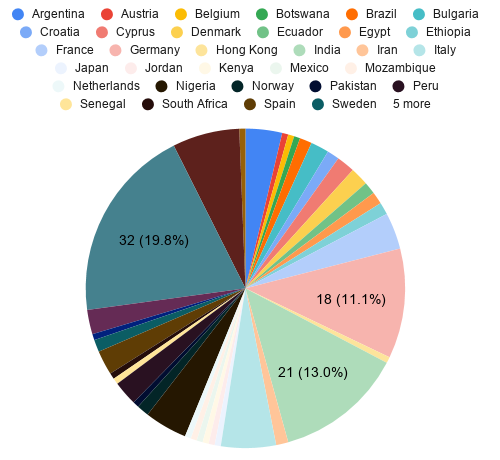
\includegraphics[scale=0.8]{country}
\caption{\label{fig:country} Country of the participants}
\end{figure}

The significant majority of the participants were PhD students (42.6\%), but we also had a substantial attendance of researchers (32.8\%), non-academic professionals, and students (not yet in PhD level) (Figure \ref{fig:occupation}).

\begin{figure}[H]
\centering
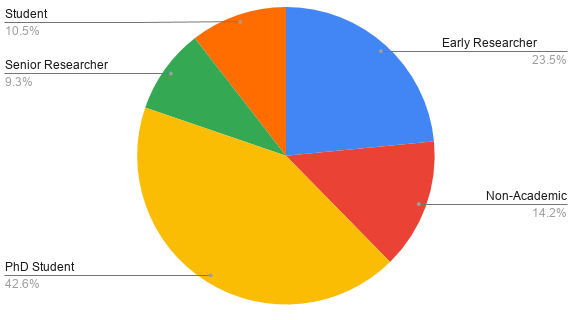
\includegraphics[scale=0.9]{occupation}
\caption{\label{fig:occupation} Occupation of the participants}
\end{figure}

In the registration form, 120 people assured they would participate in all topical sessions, and 84 would definitely participate in the hands-on sessions (Figure \ref{fig:part}).

\begin{figure}[H]
\centering
\begin{tabular}{cc}
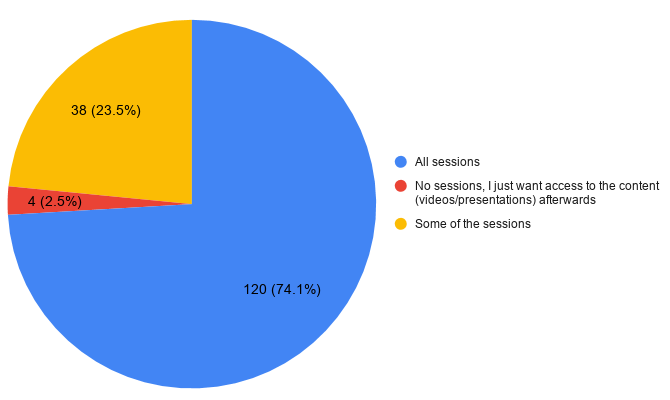
\includegraphics[scale=0.4]{sessions} &
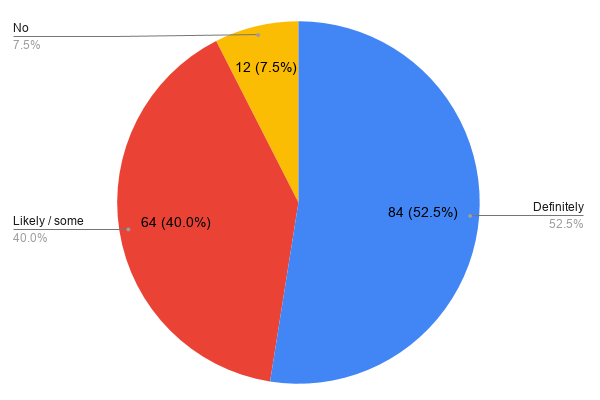
\includegraphics[scale=0.4]{hands-on} \\
\hspace{-3cm} All sessions &
Hands-on sessions
\end{tabular}
\caption{\label{fig:part} Expected participation in the summer school}
\end{figure}


The 54 people that attended more than 70\% of the event were granted a personalised certificate of participation (Figure \ref{fig:cert}).

\begin{figure}[H]
\centering
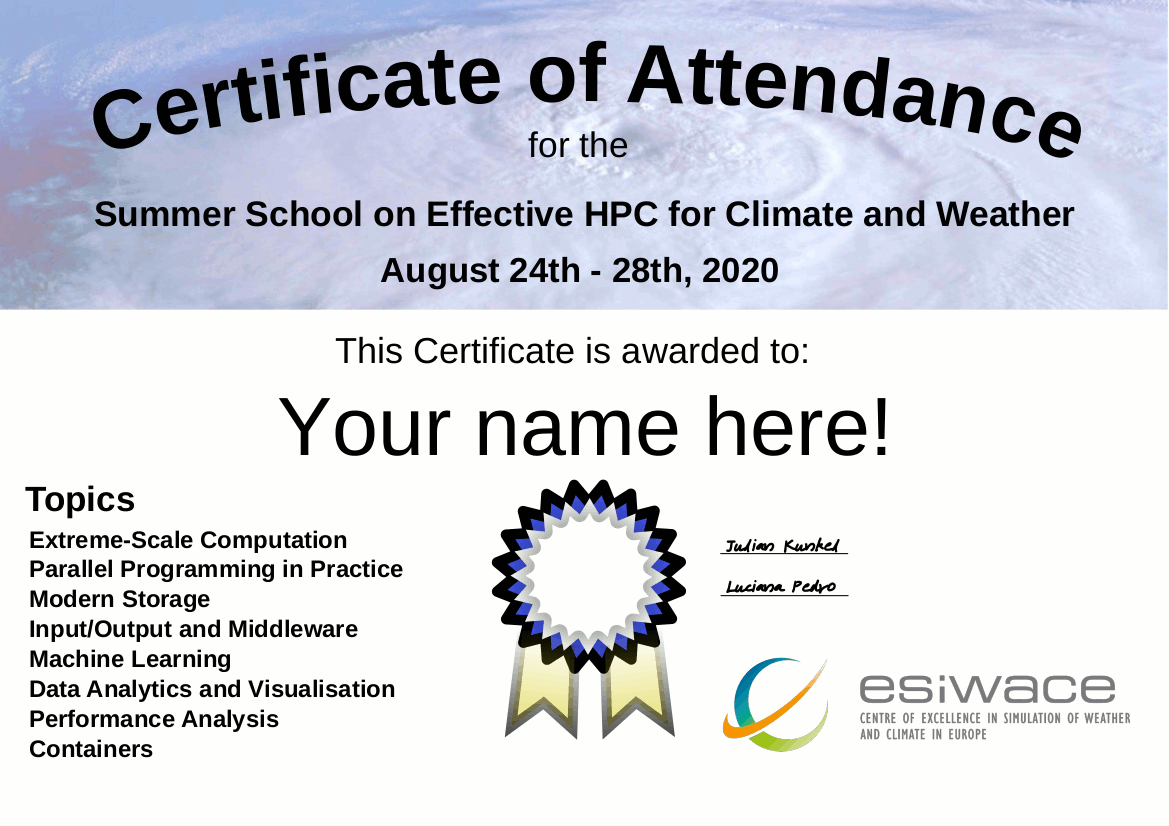
\includegraphics[scale=0.5]{certificate}
\caption{\label{fig:cert} Certificate of Attendance}
\end{figure}

\section{Survey}

After the event, we asked the participants to fulfil a \href{https://docs.google.com/forms/d/1UMMUGfos13HmsvMO6WFBrDXQkNIhOxoLooBBgoSde-I}{Survey}. The survey was sent to all participants registered in the mailing list of the event. We had 13 complete answers. The next subsections cover the statistics and the answers provided by the participants.

Here are some of the main numbers and comments about what they most liked about the summer school:

\begin{itemize}

\item 38.5\% said the summer school was better than they were expecting and 46.2\% said it was as good as they were expecting;

\item 92.3\% said they had an excellent or good experience;

\item Selected quotes from attendees:

\begin{itemize}

\item ``The combination of learning the theory, getting some hands-on it, and working with the learned things";
\item ``The interdisciplinary spirit of the presentations and profound knowledge of people invited to talk";
\item ``High-quality presentations and I can revisit it when I need on youtube".

\end{itemize}

\end{itemize}

\subsection{Statistics}

\begin{figure}[H]
\centering
\begin{tabular}{cc}
Summer School & \hspace{1cm} Blackboard Collaborate \\
\hspace{-2.5cm} 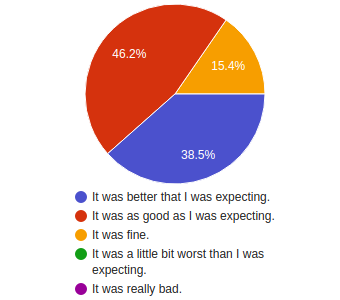
\includegraphics[scale=0.8]{survey-assessment} &
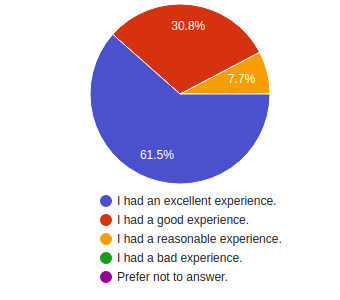
\includegraphics[scale=0.8]{survey-platform}
\end{tabular}
\caption{General assessments}
\end{figure}

\begin{figure}[H]
\centering
\begin{tabular}{cc}
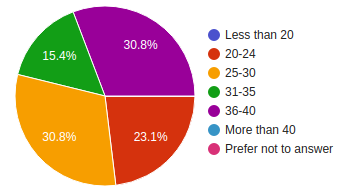
\includegraphics[scale=0.8]{survey-age} &
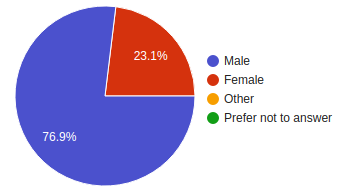
\includegraphics[scale=0.8]{survey-gender} \\
\hspace{-3.5cm} Age & \hspace{-3cm} Gender
\end{tabular}
\caption{Personal information}
\end{figure}

\begin{figure}[H]
\centering
\begin{tabular}{cc}
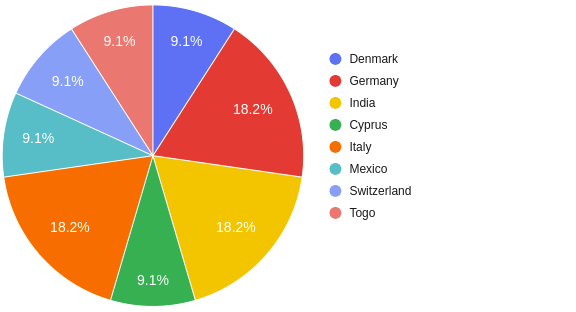
\includegraphics[scale=0.5]{survey-country} &
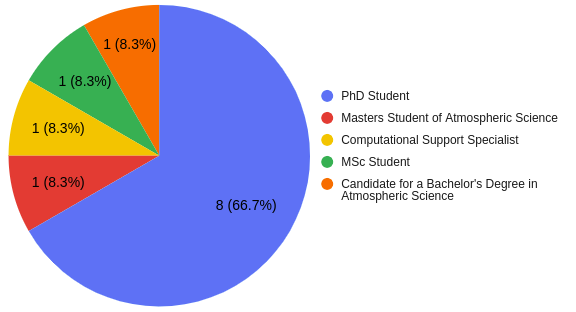
\includegraphics[scale=0.5]{survey-occupation} \\
\hspace{-4cm} Country & \hspace{-3.5cm} Occupation
\end{tabular}
\caption{Personal information}
\end{figure}

\subsection{Comments}

\subsubsection{What did you most like about the summer school?}

``High quality, great variety."

``Switching to a free online summer school instead of cancelling."

``Coupling, container, MPI."

``The combination of learning theory and get some hands-on it and work with the learned things."

``Interactive talks."

``High-quality presentations and I can revisit it when I need on youtube."

``The presentations wich application examples."

``It was new for me but very knowledgeable sessions program."

``The interdisciplinary spirit of the presentations and profound knowledge of people invited to talk."

``Practical Sessions."

``Theory as well as practical sessions."

``Feedback questions on presentation and hand-on practicals."

``I liked that it was accessible to anyone around the world. That there was a wide variety of topics and that the experts of each session were people who were passionate about their field of study. Also, everything was really good planned and that we had access to all the software in the VM."

\subsubsection{What did you most dislike about the summer school?}

``No room for personal presentation, 70 participants and no general overview or insight of who was attending from where. Also: maybe too little breaks."

``Compatibility problems with the VMs (host: mac)."

``I am not sure."

``I wasn't really into the topic before and some sessions were really hard to understand because some basic knowledge was missing."

``Hard to work online on tutorials."

``Bad English of some of the presenters."

``Time shortage in the hands-on session."

``Nothing in particular."

``None."

``Difficulty to get personalised coaching during practicals (probably due to the virtual nature of the summer school)."

``That I had to wake up at 3 AM in Mexico."

\subsubsection{Please, let a general comment about your experience in the summer school.}

``Best professionals, over a wide range, brought together into one great, interesting event."

``I've learned several things from the computational point of view. Many of which I would never even have the ability to formulate the questions if were it not for a course geared towards climate scientists."

``The introduction was quite steep and dry for a person with few knowledge about processors etc."

``It was a good experience to see some topics I am familiar with (CS) applied in an interesting field that I don't know in deep details (climate)."

``Everything was just wonderful."

``My personal experience at the summer school was great! I had a great overview of the recent advancements and orientations in HPC for the weather and climate domain."

``My experience in the course was really good. I am Mexican, and because of the time difference I had to wake up at 3 AM for the summer school, but it was totally worth it. I enjoyed every session and learned a lot. Many topics were new for me, but the speakers were excellent. It is definitely an excellent HPC introductory course and also an excellent course for those who already have some experience in the field."

\section{Improvements}

We learned many things with this first summer school that we will use to improve the event in 2021. The environment for the summer school 2021 is expected to be different (we hope we have the event in Reading, UK), but there are some lessons that we can apply to the next event, regardless of how the event will happen next year.

\begin{itemize}

\item Mailing List

It was a very good idea to create a mailing list with all participants of the event, including the speakers. However, although the list really facilitated the communication between the organisation and the attendees, the secondary benefit (support the attendees) was not achieved.

We would like that list to be used by the participants to ask questions and interact with each other and the speakers. The participants had the chat of the Blackboard Collaborate to contact the speakers during their presentation and to exchange information among themselves during the Virtual Lab Session. The former was used successfully, but the later was almost not used at all.

Encourage the attendees to use the mailing list to interact would have been an extra incentive for them to go through the recorded labs, pose different questions, help each other and extend their personal network. It was a missed opportunity that we intend to emphasise in the next summer school.

being used as a support list and to networking )

\item Networking

In the physical event, we had planned many opportunities for the participants to do networking. We had group projects and daily get together at the end of the day. When translating the event to virtual, we lost those options, and we could not think about something extra to replace the interaction they would have in the projects and confraternisations.

Here we can mention the mailing list again, that would help the attendees to contact one another and improve their personal network. Besides that, in case we need to plan another virtual event, this time we have extra time to find creative solutions for helping the participants connect to each other and also to the speakers. Hopefully, we will be able to put the original plan in practice in 2021.

\item Virtual Machine

The Virtual Machine (VM) was a fantastic idea that allowed all the participants to work with tools developed and used in ESiWACE project in the same environment. By doing that, we saved time that would be used configuring each machine and dealing with operating systems specifications. However, not everyone was able to install the VM. In this case, it was nearly impossible to follow the labs hands-on.

Again, for the event in Reading, we were planning to have physical labs in which the system would be already appropriately configured for all the attendees to focus their attention only in the tools they are learning, and not waste time configuring systems. But even in a physical event, the VM is a good idea because it allows the participants to practice on their own and in their personal machine.

The VM was delivered to the participants a month in advance, to give them time to fix any possible incompatibility with their machine. For the event in 2021, we plan on having the VM again, together with a dedicated assistant (possibly one of Reading's students) to provide support for the participants that are facing problems that they cannot solve. With that, we intend to guarantee that everyone will have the VM adequately installed and running, and they will then have the opportunity to attend all labs prepared for the event.

\item Survey

From the survey, we also noticed further room for improvements:

\begin{itemize}

\item ``No room for personal presentation, 70 participants and no general overview or insight of
who was attending from where."

We hope to have a better networking structure in the next event.

\item ``Maybe too little breaks."

We had a structure with 15 minutes break during the morning and afternoon sessions and 45 minutes for a lunch break. The small duration of the intervals is standard in this kind of event, and we took advantage of the virtual structure to have a more compact lunch break. If we need to run the event online again, we may rethink these options. If a physical event is possible in 2021, the whole structure will change, and we will address the breaks more carefully.

\item ``Time shortage in the hands-on session."

The hands-on sessions were pre-recorded to give the participants the freedom to choose which session to check out. Again, modifications in the format will depend on the kind of event we can organise in 2021.

\item ``Difficulty to get a personalised coaching during practicals (probably due to the virtual
nature of the summer school)."

When we were planning the event, we had designed group projects. In this case, each group of four to five people would have a designated supervisor. With the virtual event, the number of participants was too high to have personalised coaching. But many of the speakers left their contacts and offered to provide further help during and after the event.

\item ``That I had to wake up at 3 AM of Mexico."

We hope to welcome all the participants in Reading (UK) for the summer school in 2021. Hence everyone can attend the sessions in reasonable hours.

\end{itemize}

\end{itemize}
